\documentclass[conference]{IEEEtran}
\usepackage{cite}
\usepackage{amsmath,amssymb,amsfonts}
\usepackage{algorithmic}
\usepackage{graphicx}
\usepackage{textcomp}
\usepackage{xcolor}
\usepackage{booktabs}
\usepackage{multirow}
\usepackage{float}
\usepackage{hyperref}

\def\BibTeX{{\rm B\kern-.05em{\sc i\kern-.025em b}\kern-.08em
    T\kern-.1667em\lower.7ex\hbox{E}\kern-.125emX}}

\begin{document}

\title{DPCR-IDS: A Lightweight Dual-Protocol Cascade Routing Intrusion Detection System for Automotive Networks}

\author{\IEEEauthorblockN{Anonymous Authors}
\IEEEauthorblockA{\textit{Affiliation}\\
City, Country \\
email@domain.com}
}

\maketitle

\begin{abstract}
Modern automotive systems are complex networks comprising numerous Electronic Control Units (ECUs) communicating over fundamentally different protocols, notably CAN Bus and Automotive Ethernet. While legacy protocols like CAN lack built-in security, newer Ethernet networks face sophisticated threats such as frame injection and spoofing. Existing Intrusion Detection Systems (IDS) generally focus on a single protocol, rendering them blind to cross-protocol and complex attacks, or they rely on heavy deep learning models unsuitable for resource-constrained automotive edge hardware. In this paper, we propose DPCR-IDS (Dual-Protocol Cascade Routing IDS), a novel architecture that monitors both CAN and Automotive Ethernet simultaneously. DPCR-IDS employs a two-tier knowledge distillation cascade to compress heavy Transformer-based teachers into lightweight CNN and TCN student models. A confidence-based routing mechanism with an expert-aware override directs ambiguous samples to a late-fusion gated multi-layer perceptron, while 99.3\% of traffic is classified in the sub-millisecond fast path. Evaluation on the Car-Hacking and TOW-IDS datasets demonstrates high accuracy, achieving 99.97\% detection rate for CAN attacks and a 95.98\% cross-protocol fusion F1 score, with a total edge deployment footprint of just 52,757 parameters. Furthermore, discrete-event network simulation in OMNeT++ using real ONNX Runtime inference validates the system's compliance with strict 20 ms automotive processing deadlines.
\end{abstract}

\begin{IEEEkeywords}
Intrusion Detection, Automotive Security, CAN Bus, Automotive Ethernet, Knowledge Distillation, Sensor Fusion, Edge Computing
\end{IEEEkeywords}

\section{Introduction}
Modern vehicles have evolved into complex networked cyber-physical systems containing 70 to over 100 Electronic Control Units (ECUs). These ECUs communicate over multiple network protocols to support functionalities ranging from powertrain control to Advanced Driver Assistance Systems (ADAS). Two of the most prominent protocols in contemporary architectures are the Controller Area Network (CAN) and Automotive Ethernet.

The CAN Bus, developed in the 1980s, is the de facto standard for critical vehicle operations. However, it was designed without fundamental security mechanisms like authentication or encryption. Consequently, if an attacker gains access to the bus, they can easily execute spoofing, fuzzing, or Denial-of-Service (DoS) attacks \cite{can_sec}. Conversely, Automotive Ethernet provides the high bandwidth (100 Mbps to 10 Gbps) required for modern ADAS and infotainment systems. While IP-based protocols offer more security features, they introduce a broader attack surface, making the network vulnerable to packet injection, MAC flooding, and credential replay.

As vehicle architectures shift toward centralized and zonal computing via powerful gateway ECUs, attacks often span across multiple bus segments. For instance, a compromised infotainment unit on an Ethernet network may attempt to spoof gear control messages on the CAN bus. Existing Intrusion Detection Systems (IDS) predominantly address a single protocol, rendering them ineffective against coordinated, cross-protocol attacks. Furthermore, proposed deep learning (DL) solutions often rely on computationally intensive architectures (e.g., Transformers or LSTMs) that cannot be deployed on resource-constrained automotive gateways operating under strict latency constraints (e.g., $<20$ ms).

To bridge this gap, we present the Dual-Protocol Cascade Routing Intrusion Detection System (DPCR-IDS). DPCR-IDS is designed for edge deployment on automotive gateways, simultaneously monitoring CAN and Ethernet traffic. By leveraging a teacher-student knowledge distillation approach, we significantly reduce the parameter footprint of the detection models. Additionally, we introduce a novel confidence-based routing mechanism equipped with an expert-aware override and a Random Forest fallback, ensuring that the computationally heavier fusion head is only activated for ambiguous traffic.

The key contributions of this paper are:
\begin{enumerate}
    \item A unified, dual-protocol IDS covering both CAN and Automotive Ethernet with an aggregated decision framework.
    \item A two-tier distillation cascade that compresses the models by approximately $30\times$ compared to the teacher baseline, achieving a total edge deployment size of 52,757 parameters.
    \item A confidence-based routing architecture with a late decision fusion mechanism that processes over 99\% of traffic via a sub-millisecond fast path.
    \item Comprehensive evaluation using both offline machine learning metrics and network-level discrete-event simulation (OMNeT++) with real ONNX Runtime integration.
\end{enumerate}

\section{Related Work}
\subsection{Single-Protocol Intrusion Detection}
Extensive research has addressed intrusion detection for the CAN bus. Approaches range from statistical and frequency-based analysis to deep learning methods such as Convolutional Neural Networks (CNN) and Recurrent Neural Networks (RNN) \cite{can_dl}. While these models achieve high accuracy on datasets like the Car-Hacking dataset, they ignore the broader vehicle network.
Similarly, Ethernet-based IDSs have adapted IT network security techniques to the automotive domain. Recent works utilize payload inspection and flow-based features \cite{eth_ids}. However, these approaches remain isolated from the vehicle's cyber-physical state monitored by CAN.

\subsection{Multi-Protocol and Edge IDS}
Literature on multi-protocol automotive IDS is sparse. Most gateway solutions rely on rigid rule-based routing or independent processing pipelines without genuine cross-protocol fusion. Furthermore, deploying advanced DL models on edge devices like automotive gateways is hindered by strict resource limits. Knowledge distillation has emerged as a promising technique to compress large models for edge deployment, but its application in a multi-protocol, cascading routing architecture for vehicles remains unexplored.

\section{System Architecture}

\subsection{System Overview}
DPCR-IDS operates on the gateway ECU, monitoring ingress traffic from both CAN and Ethernet buses. The system is designed around a cascading architecture comprising independent protocol experts, a confidence router, a fallback classifier, and a late-fusion head. The architecture ensures that unambiguous, benign traffic is processed rapidly, while suspicious or complex patterns are escalated.

\subsection{Feature Engineering and Extraction}
\textbf{CAN Bus:} To capture both raw payload anomalies and temporal attack patterns (e.g., DoS flooding), the CAN feature extractor processes windows of 100 consecutive frames (stride of 50). It extracts 16 features per frame, including normalized ID, Data Length Code (DLC), 8 payload bytes, and 6 engineered temporal/statistical features (e.g., Inter-Arrival Time (IAT), payload entropy, message frequency, and bitflip ratio).

\textbf{Automotive Ethernet:} For Ethernet, we adopt a byte-image encoding strategy. The first 1024 bytes of the payload are mapped into a $32\times 32$ matrix with 4 channels, preserving spatial locality of packet structures without requiring deep protocol dissection.

\subsection{Knowledge Distillation Cascade}
To satisfy edge constraints, we employ knowledge distillation. Large Transformer-based teacher models (approx. 3.2M parameters each) are trained offline to generate soft labels. 

The student models are trained using a combined loss function:
\begin{equation}
L_{total} = \alpha L_{distill}(z_s, z_t, T) + (1-\alpha)L_{BCE}(z_s, y)
\end{equation}
where $z_s$ and $z_t$ are student and teacher logits, $T$ is the temperature, and $y$ is the hard label.
\begin{itemize}
    \item \textbf{CAN Student:} A Depthwise-Separable Temporal Convolutional Network (TCN) with 22,977 parameters.
    \item \textbf{Ethernet Student:} A lightweight 2D CNN with 28,321 parameters.
\end{itemize}
Both models output a single attack logit and a 128-dimensional embedding.

\subsection{Confidence Routing and Late Fusion}

\begin{figure}[H]
\centering
\includegraphics[width=0.48\textwidth]{../artifacts/dpcr_ids_research_v1/paper_figures/fig_router_flowchart.png}
\caption{DPCR-IDS Confidence Routing and Flow Architecture.}
\label{fig:router_flowchart}
\end{figure}

The \textbf{Confidence Router} efficiently dictates the processing path based on the post-calibrated prediction probabilities ($p$) of the independent experts. We define thresholds $\tau_{low} = 0.15$ and $\tau_{high} = 0.85$.
\begin{itemize}
    \item If $p < \tau_{low}$, the traffic is classified as NORMAL (Fast Path).
    \item If $p > \tau_{high}$, it is classified as ATTACK (Fast Path).
    \item If $\tau_{low} \leq p \leq \tau_{high}$, the sample is deemed ambiguous.
\end{itemize}

\textbf{Expert-Aware Override:} To mitigate false positives in entirely benign scenarios, if all individual experts predict NORMAL with high confidence, the router overrides and outputs NORMAL, bypassing further escalation.

For ambiguous samples entering the heavy path, a \textbf{Random Forest Fallback} classifier processes the 128-d embeddings. If uncertainty persists, the sample is escalated to the \textbf{Late Fusion Head}. This head is a Tiny Gated Multi-Layer Perceptron (MLP) containing just 1,459 parameters. It learns per-expert attention weights, allowing dynamic trust assignment before final classification. Decisions are then merged in a 250\,ms \textbf{Decision Aggregator} bucket.

\section{Experimental Setup}

\subsection{Datasets}
We utilize two publicly available datasets:
\begin{itemize}
    \item \textbf{CAN Bus:} The Car-Hacking Dataset \cite{car_hacking}, containing DoS, Fuzzy, Gear Spoofing, and RPM Spoofing attacks.
    \item \textbf{Automotive Ethernet:} The TOW-IDS Dataset, featuring connection drops, resets, frame injection, and malformed packets.
\end{itemize}
Data is split temporally (70\% train, 15\% validation, 15\% test) to prevent data leakage.

\subsection{Evaluation Metrics}
To evaluate model performance, we report Precision (the ratio of correct attack predictions to total attack predictions), Recall or Detection Rate (the ratio of correctly detected attacks to actual attacks), and False Positive Rate (FPR, the ratio of benign traffic incorrectly classified as attacks). Additionally, model calibration is measured using Expected Calibration Error (ECE) \cite{ece_paper}, defined as:
\begin{equation}
ECE = \sum_{m=1}^{M} \frac{|B_m|}{n} |acc(B_m) - conf(B_m)|
\end{equation}
where $M$ is the number of bins, $n$ is total samples, $B_m$ is the $m$-th bin, $acc(B_m)$ is the accuracy in bin $m$, and $conf(B_m)$ is the average confidence in bin $m$.

\subsection{Implementation and Edge Deployment}
Models are implemented in PyTorch and exported to ONNX format. The complete edge deployment comprises only 52,757 parameters (CAN: 22,977; ETH: 28,321; Fusion: 1,459). The ONNX models occupy approximately 212 KB of storage, making them suitable for ARM-based gateways (e.g., Raspberry Pi 5).

\subsection{Network Simulation Framework}
To validate real-time viability, we constructed a discrete-event network simulation using OMNeT++ (v6.3.0) \cite{omnetpp}. The simulation links the ONNX Runtime (v1.17.0) \cite{onnx} C++ library to execute the exact exported models within the gateway node. We evaluated 12 configurations spanning varied attack types, bus loads (20\% to 80\%), and ECU scaling (5 to 20 nodes).

\section{Results}

\subsection{Expert Model Performance}
Following distillation and temperature scaling calibration, the models achieved exceptional unimodal performance on the held-out test sets (Table \ref{tab:expert_performance}). The CAN TCN achieved a 99.97\% Detection Rate (DR) with near-zero false positives. 

\begin{table}[H]
\centering
\caption{Expert Student Performance (Test Set)}
\label{tab:expert_performance}
\begin{tabular}{lcc}
\toprule
\textbf{Metric} & \textbf{CAN (TCN)} & \textbf{Ethernet (CNN)} \\
\midrule
Precision & 99.99\% & 91.95\% \\
Recall (DR) & 99.97\% & 68.51\% \\
F1 Score & 99.98\% & 78.52\% \\
FPR & 0.01\% & 1.19\% \\
AUC-PR & 0.9999 & 0.8927 \\
\bottomrule
\end{tabular}
\end{table}

A breakdown by attack type revealed that the Ethernet recall was impacted entirely by a 3.13\% DR on the ``CAN DoS Tunneled'' attack within TOW-IDS, as the payload image representation lacks the temporal context required to detect encapsulated CAN floods. All other Ethernet attacks achieved $>99.3\%$ DR.

\begin{table}[H]
\centering
\caption{Distillation Ablation (Validation Set)}
\label{tab:ablation}
\resizebox{\columnwidth}{!}{%
\input{../artifacts/dpcr_ids_research_v1/paper_tables/distillation_ablation.tex}
}
\end{table}

\subsection{Per-Attack-Type Performance}
To understand the models' detection capabilities across distinct threat vectors, we detail the detection performance per attack type in Table \ref{tab:can_per_attack} and Table \ref{tab:eth_per_attack}.

\begin{table}[H]
\centering
\caption{CAN Performance per Attack Type}
\label{tab:can_per_attack}
\input{../artifacts/dpcr_ids_research_v1/paper_tables/can_per_attack_type.tex}
\end{table}

\begin{table}[H]
\centering
\caption{Ethernet Performance per Attack Type}
\label{tab:eth_per_attack}
\input{../artifacts/dpcr_ids_research_v1/paper_tables/ethernet_per_attack_type.tex}
\end{table}

\subsection{Cascade and Routing Efficiency}
The fusion model achieved an F1 score of 95.98\% on cross-protocol paired data. Crucially, the confidence router successfully triaged the vast majority of traffic. In a dense multi-attack simulation scenario, 99.3\% of all decisions were resolved on the fast path, activating the fusion head for only 0.7\% of the windows.

\subsection{Complexity and Inference Latency}
Table \ref{tab:complexity} outlines the computational efficiency of the system. The entire edge pipeline requires only 232 KB of parameters. 
Inference latency benchmarking (CPU) demonstrated end-to-end execution times well below the 20\,ms budget: the CAN pipeline averaged 0.997\,ms, Ethernet 0.721\,ms, and the isolated fusion ONNX model executed in 0.005\,ms.

\begin{table}[H]
\centering
\caption{Model Complexity and Parameters}
\label{tab:complexity}
\input{../artifacts/dpcr_ids_research_v1/paper_tables/model_complexity.tex}
\end{table}

\subsection{Network Simulation Results}
The OMNeT++ simulations validated the resilience of the architecture. Under high bus load congestion (80\%), the 99th percentile end-to-end processing latency remained under 3.6\,ms. The system successfully aggregated alerts within the required 250\,ms window across all scenarios, missing zero deadlines. The expert-aware override effectively mitigated baseline false positives, maintaining a 0\% FPR in normal driving simulations.

Table \ref{tab:sim_latency} details the end-to-end inference latency results across different threat scenarios, corresponding to the visual representation in Figure \ref{fig:e2e_latency}.

\begin{table}[H]
\centering
\caption{Simulation Inference Latency (Mean $\pm$ Max, ms)}
\label{tab:sim_latency}
\resizebox{\columnwidth}{!}{%
\input{../artifacts/dpcr_ids_research_v1/paper_tables/simulation_latency.tex}
}
\end{table}

\begin{figure}[H]
\centering
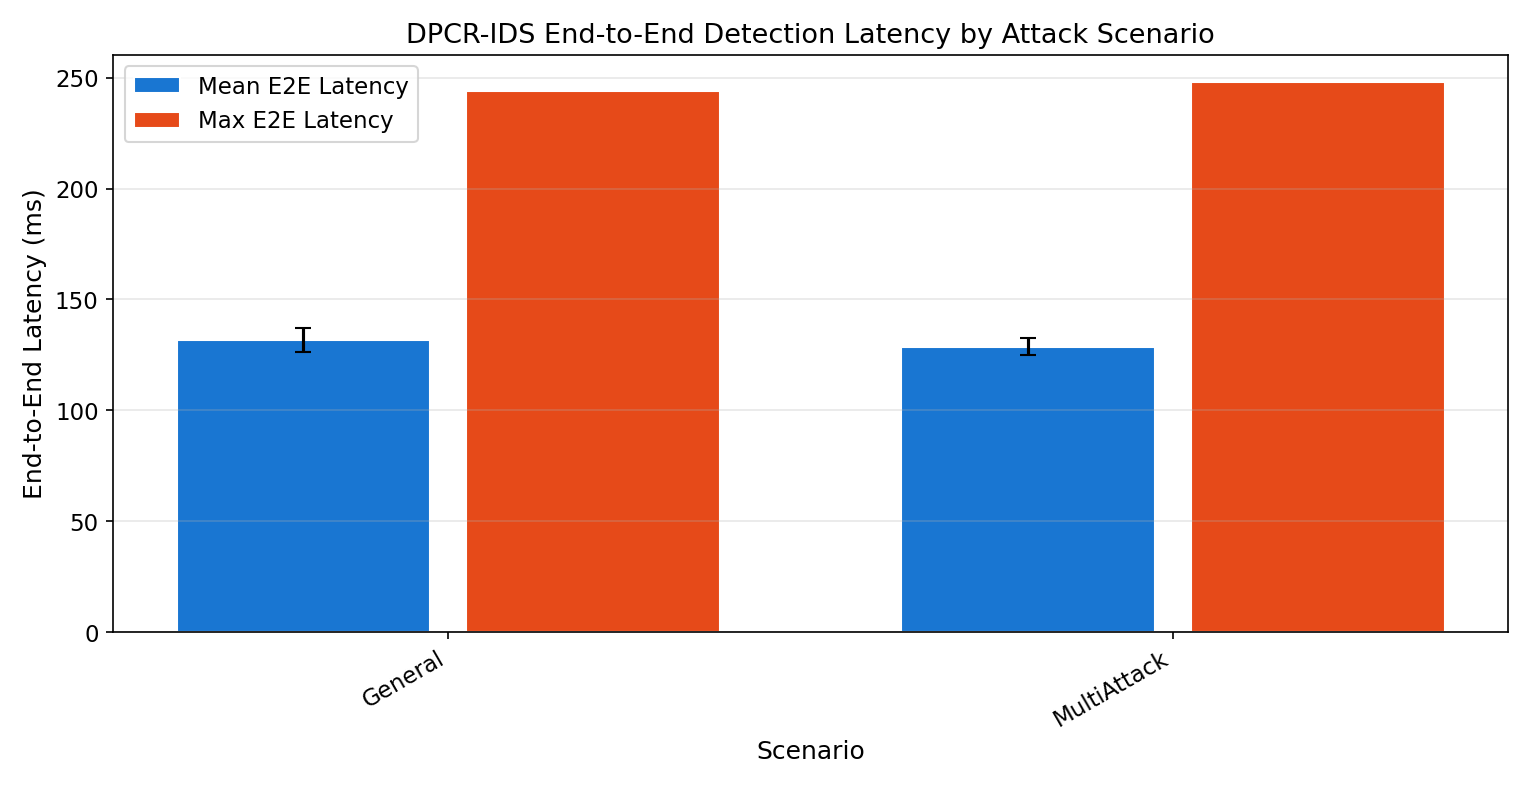
\includegraphics[width=0.48\textwidth]{../dpcr-ids-sim/simulations/results/figures/fig1_e2e_latency_attacks.png}
\caption{End-to-End Latency vs Threat Scenarios.}
\label{fig:e2e_latency}
\end{figure}

\begin{figure}[H]
\centering
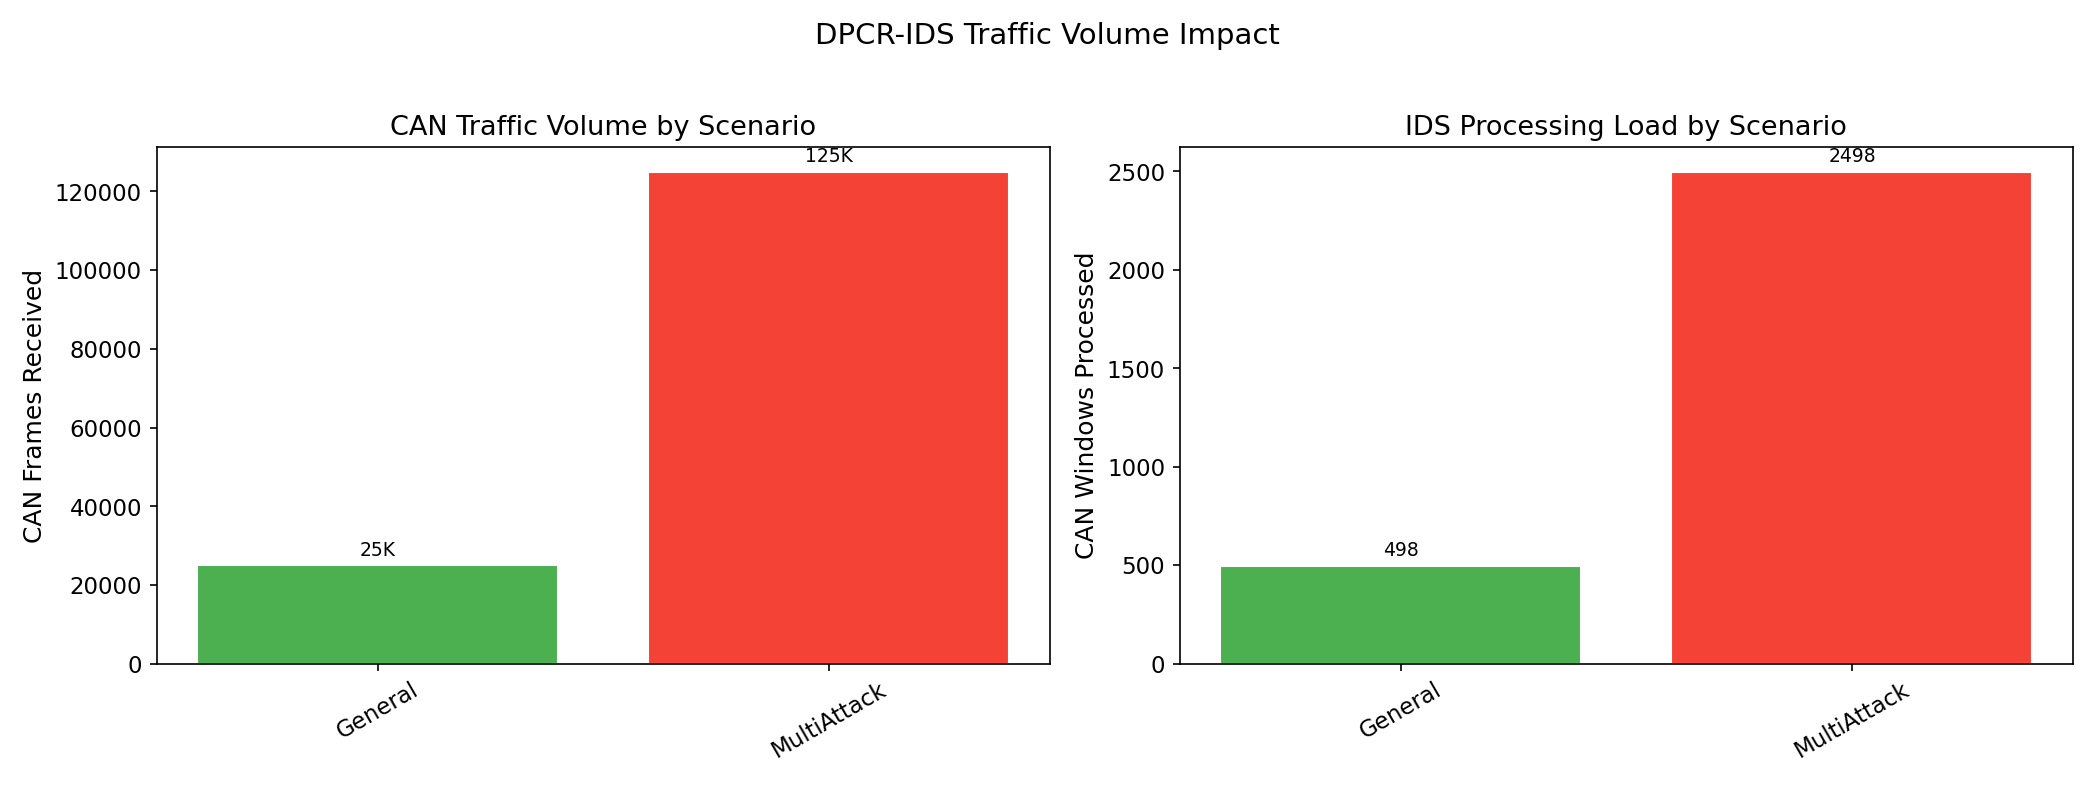
\includegraphics[width=0.48\textwidth]{../dpcr-ids-sim/simulations/results/figures/fig2_traffic_volume.png}
\caption{Total Processed Traffic Volume across Scenarios.}
\label{fig:traffic_volume}
\end{figure}

\begin{figure}[H]
\centering
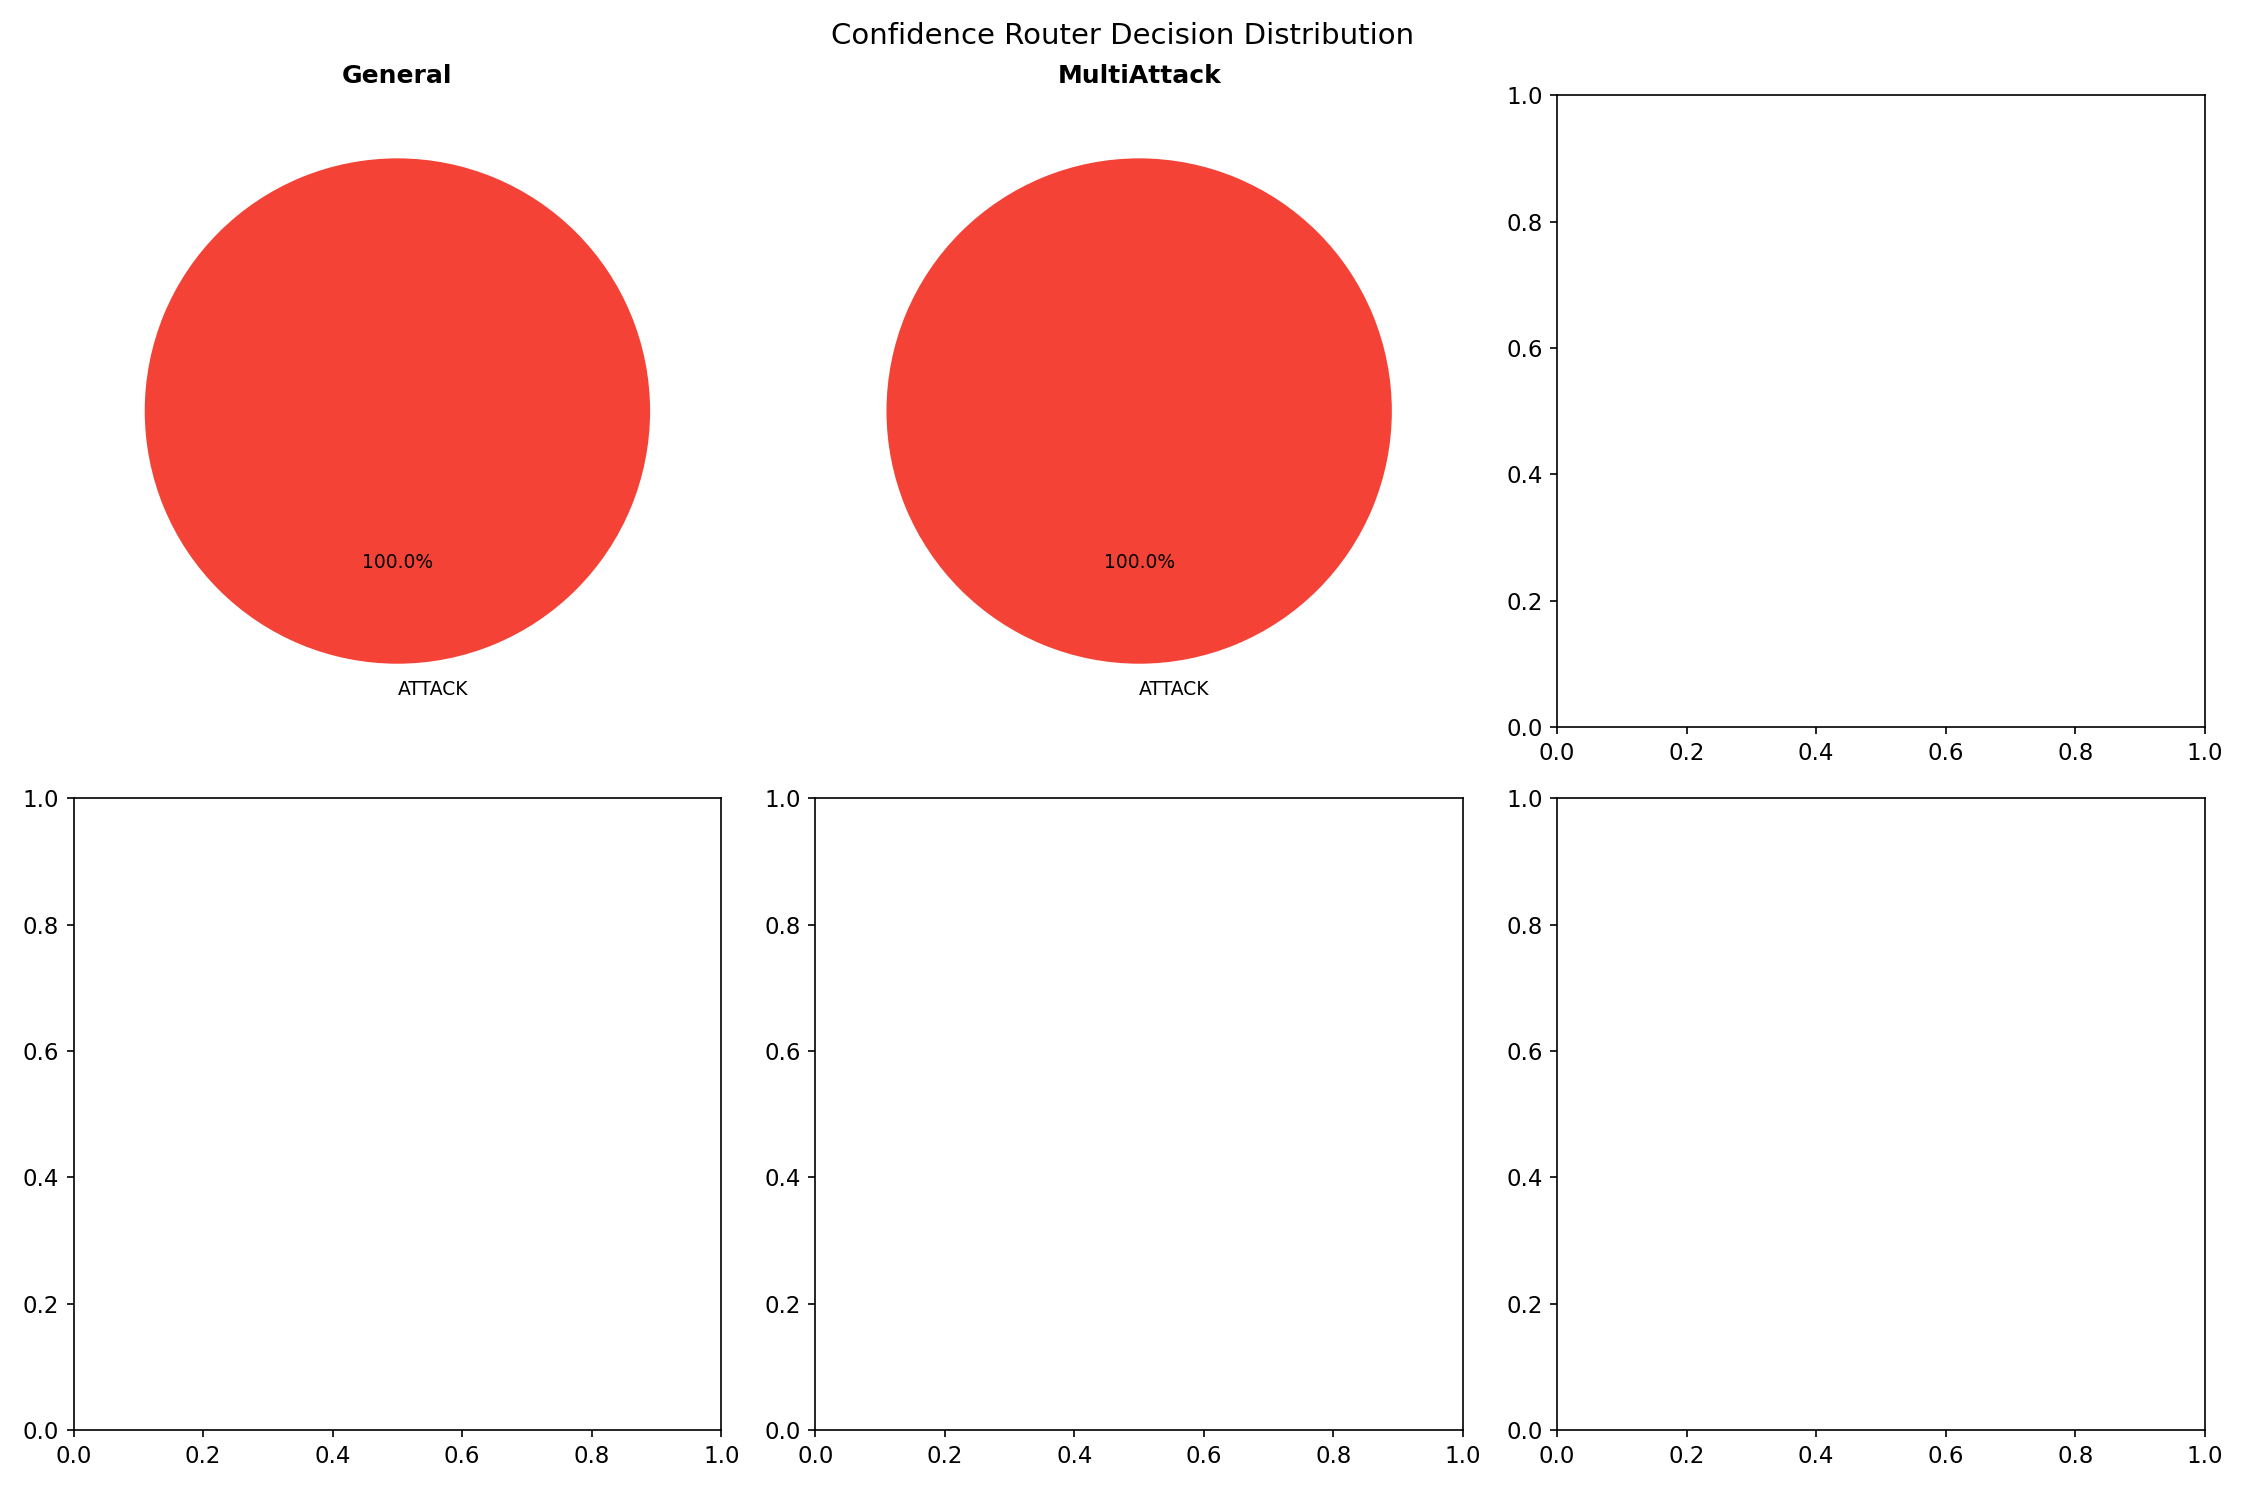
\includegraphics[width=0.48\textwidth]{../dpcr-ids-sim/simulations/results/figures/fig3_routing_decisions.png}
\caption{Network Traffic Routing Decisions.}
\label{fig:routing_decisions}
\end{figure}

\begin{figure}[H]
\centering
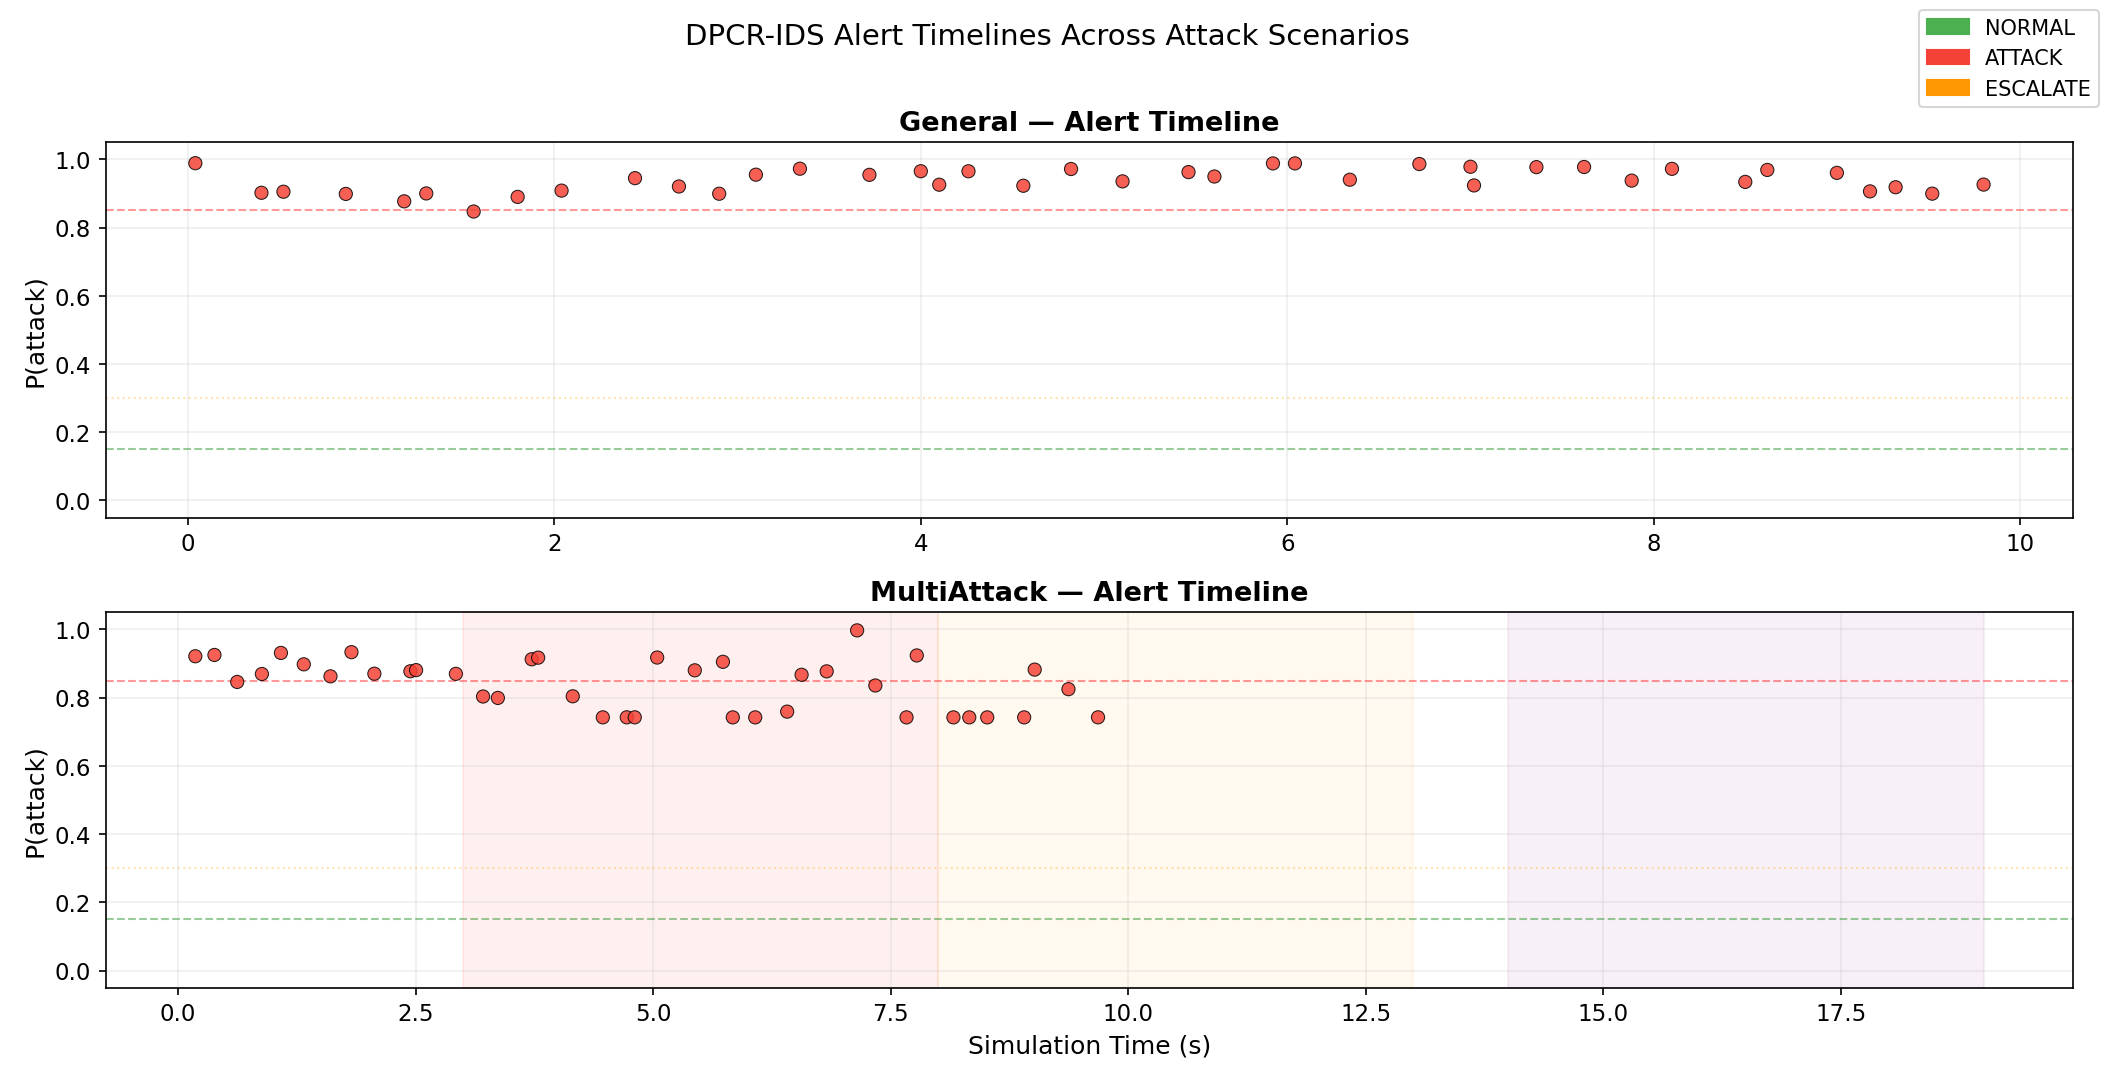
\includegraphics[width=0.48\textwidth]{../dpcr-ids-sim/simulations/results/figures/fig4_alert_timelines.png}
\caption{System Alert Timelines.}
\label{fig:alert_timelines}
\end{figure}

\section{Discussion}
DPCR-IDS addresses the critical need for unified, resource-efficient automotive security. By relying heavily on the fast path, the architecture achieves a high overall detection rate without the computational bottleneck of continuous sensor fusion. 

A recognized limitation is the Ethernet model's low detection rate for tunneled CAN DoS attacks. Because the Ethernet CNN processes spatial payload representations independently, it lacks the inter-arrival time metrics explicitly engineered into the CAN pipeline. Future work will investigate embedding temporal or flow-based features into the Ethernet path to resolve this blind spot, and testing the system against adaptive adversarial attacks.

\section{Conclusion}
This paper presented DPCR-IDS, a dual-protocol cascade routing IDS for next-generation automotive networks. Through teacher-student distillation and a novel confidence-based routing mechanism, we achieved a $30\times$ reduction in model parameters compared to standalone deep networks, rendering the system suitable for embedded gateway deployment. Experimental results and OMNeT++ simulations demonstrate that DPCR-IDS maintains high detection accuracy across diverse attack vectors while strictly adhering to the sub-20\,ms latency requirements of automotive cyber-physical systems.

\section{Data and Code Availability}
The code and models used in this research are available in the public repository to facilitate reproducibility and future advancements in automotive security.

\begin{thebibliography}{00}
\bibitem{can_sec} A. Bozdal, M. Samie, S. Aslam, and I. Jennions, ``Evaluation of CAN Bus Security Challenges,'' \emph{Sensors}, vol. 20, no. 8, p. 2364, 2020.
\bibitem{can_dl} H. Lee, S. H. Jeong, and H. K. Kim, ``OTIDS: A novel intrusion detection system for in-vehicle network by using timing-based anomaly detection,'' \emph{11th International Conference on Availability, Reliability and Security (ARES)}, 2017.
\bibitem{eth_ids} M. Wolf, A. Weimerskirch, and C. Paar, ``Security in Automotive Bus Systems,'' \emph{Workshop on Embedded Security in Cars}, 2004.
\bibitem{car_hacking} M.-J. Kang and J.-W. Kang, ``Intrusion detection system using deep neural network for in-vehicle network security,'' \emph{PLoS ONE}, vol. 11, no. 6, 2016.
\bibitem{ece_paper} M. P. Naeini, G. Cooper, and M. Hauskrecht, ``Obtaining well calibrated probabilities using bayesian binning,'' \emph{Twenty-Ninth AAAI Conference on Artificial Intelligence}, 2015.
\bibitem{omnetpp} A. Varga, ``The OMNeT++ discrete event simulation system,'' \emph{Proceedings of the European Simulation Multiconference (ESM)}, 2001.
\bibitem{onnx} J. Bai et al., ``ONNX: Open Neural Network Exchange,'' \emph{GitHub repository}, 2019.
\end{thebibliography}

\end{document}
